\section{Data Analysis}
With the data I collected, a total of 56 participants were involved in my research study - giving me a total of 560 results to analyse (280 per stage). This data collected was then split into two separate CSV files holding the appropriate data regarding each stage. The data was used in a series of Binomial Tests in R (See \hyperref[append:g]{\italic{Appendix G}}) and appropriate charts were generated to visualise the data in each stage (See Fig~\ref{stage-1-graph} and Fig~\ref{stage-2-graph}).

\subsection{Hypothesis Results}
\subsubsection{Hypothesis 1}
The first hypotheses;
\textit{When unaware, the Artefact (M-A System) is picked more often than Human designed interiors by participants}.

\subsubsection{Hypothesis 2}
blah blah blah results. failed to reject null hypothesis.

\begin{figure}[!ht]
    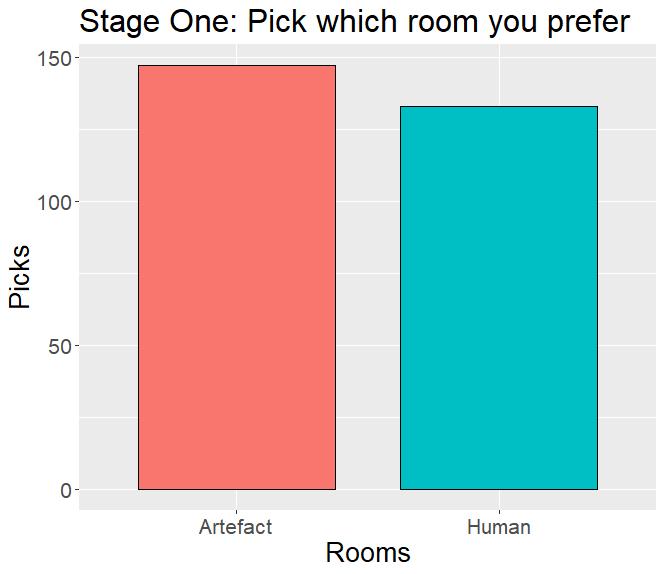
\includegraphics[width=\columnwidth]{./Images/stage-1-picks-graph.png}
    \centering
    \caption{Bar chart representing the data from Stage 1}
    \label{stage-1-graph}
\end{figure}

\begin{figure}[!ht]
    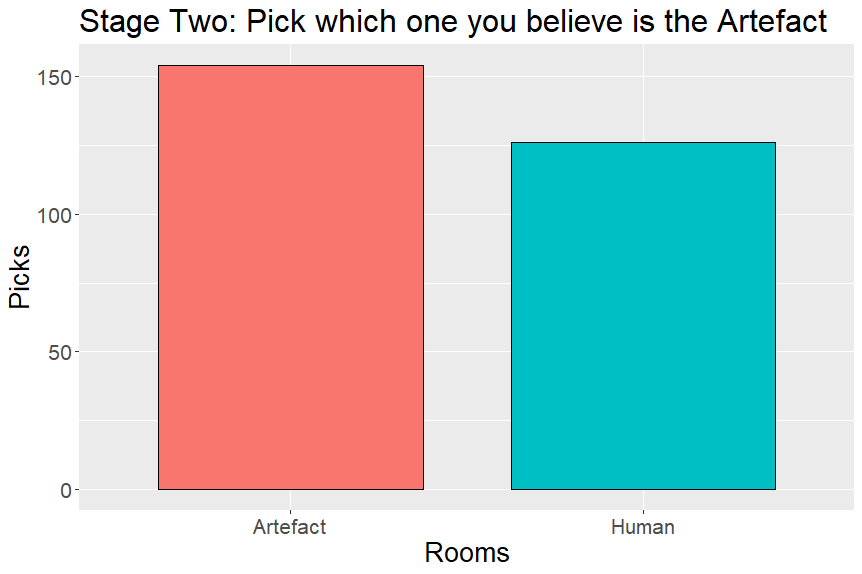
\includegraphics[width=\columnwidth]{./Images/stage-2-picks-graph.png}
    \centering
    \caption{Bar chart representing the data from Stage 2}
    \label{stage-2-graph}
\end{figure}